\documentclass{article}
\title{CMSC 471 Project 2}
\author{Zach Long}
\date{March 18, 2015}
\usepackage{graphicx}
\begin{document}
   \maketitle
   \section{Hill Climbing}
   Our simplest and most basic optimization method. While it is the fastest of the three, it is the most unreliable. First we pick a random point in the given domain, look at the eight cardinal and intermediate directions that are stepsize away from our point, and take the smallest of those, making this implementation steepest ascent hill climbing, and then look at it's neighbors. We continue the process until we find a local minimum.

   \begin{figure}[h!]
      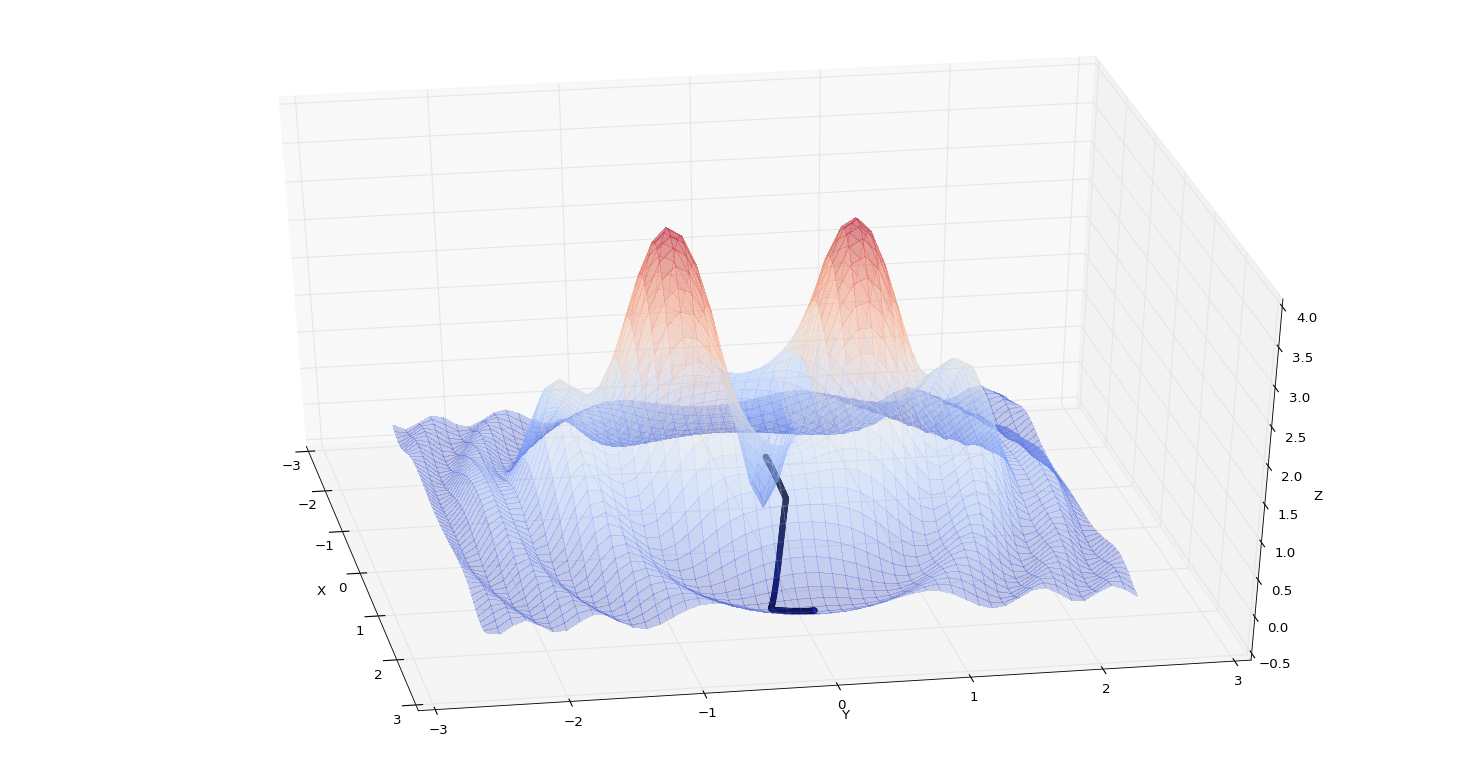
\includegraphics[width=\linewidth]{hill_climb.png}
      \caption{Hill climbing with step size .001}
      \label{fig:graph1}
   \end{figure}

   \section{Hill Climbing With Random Restarts}
   A simple modification to our Climbing algorithm, we simply loop through it numrestarts times and return the smallest point between all of them. From my experience, I have found this to be the most effective of the three methods in finding the global minimum of the function, although it does take a noticeable amount of time longer. Obviously this will be significantly better than Hill Climbing, as throwing 100 darts at a board and you're much more likely to hit the right spot than just throwing one. It also does better than simulated annealing, who's issues we'll look at next.

   \begin{figure}[h!]
      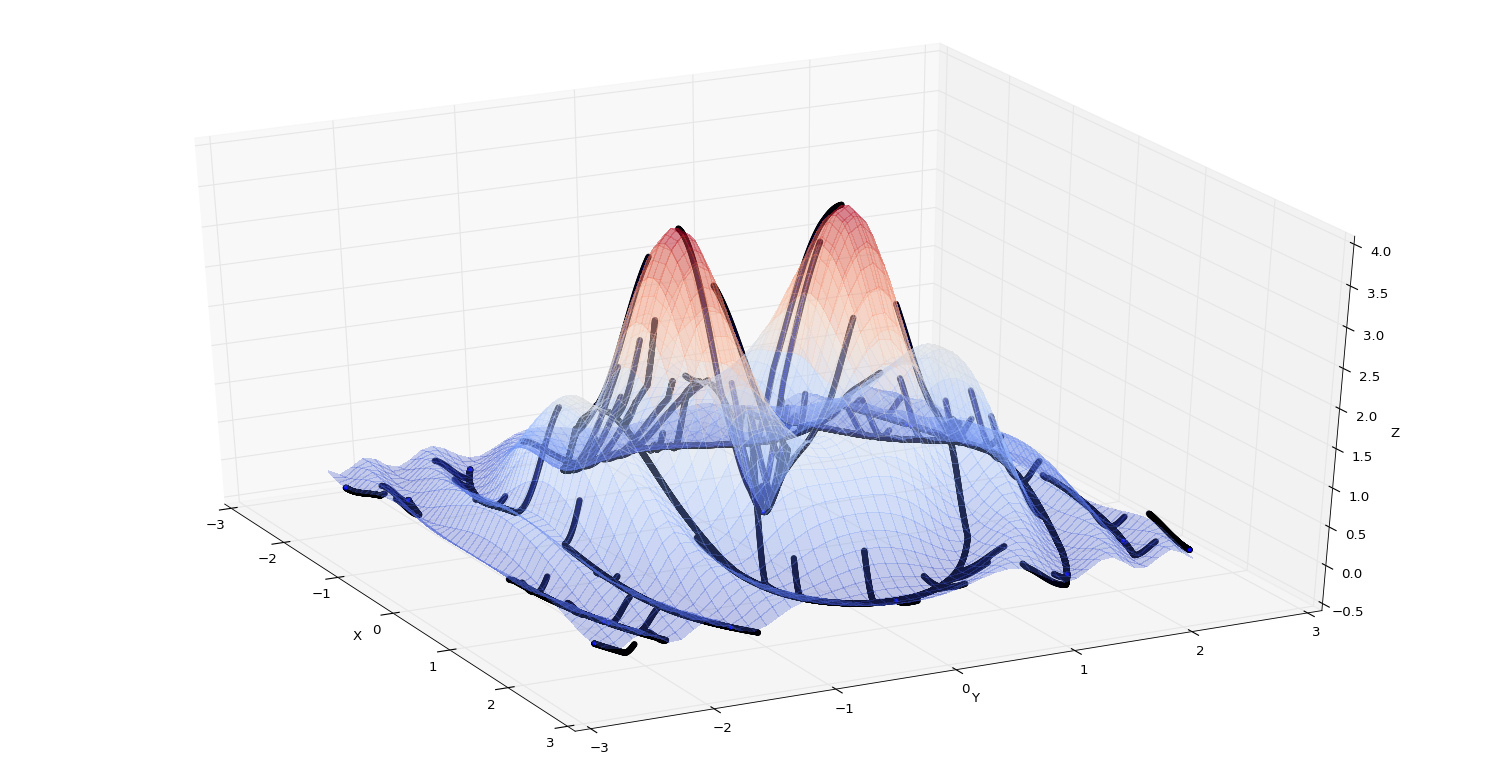
\includegraphics[width=\linewidth]{hill_climb_restarts.png}
      \caption{Hill climbing with step size .001 and 100 restarts}
      \label{fig:graph2}
   \end{figure}

   \section{Simulated Annealing}
   The actually interesting optimization algorithm! We take a random point, then take another random point inside the neiborhood of radius step size, and if it is less than our original point, move there. If it isn't though, there is a \(e^{-(newZ - currentZ) / temperature} \) chance that we move there anyway, meaning that as the temperature decreases we become hill climbing, but until then we are capable of moving over local minima. Once the temp is low enough, or our point is unchanged for 100 iterations, we return the best point we found. It runs a bit slower than basic hill climbing, but is more reliable for it's ability to break out of pits. However, it doesn't manage to be as consistent as hill climbing with 100+ random restarts. Reasoning for that could be in the various options that simulated annealing has. Various neiborhood sizes, whether to have the neighborhood size be static or scale down with the temperature, and  how we lower the temperature all contribute to how successful simulated annealing ends up being, and they should be tailored for each individual function you wish to minimize. So, there may be some combination of those that leads to more consistent min finding with this function, but unfortunately I was unable to find it with my tinkering.

   \begin{figure}[h!]
      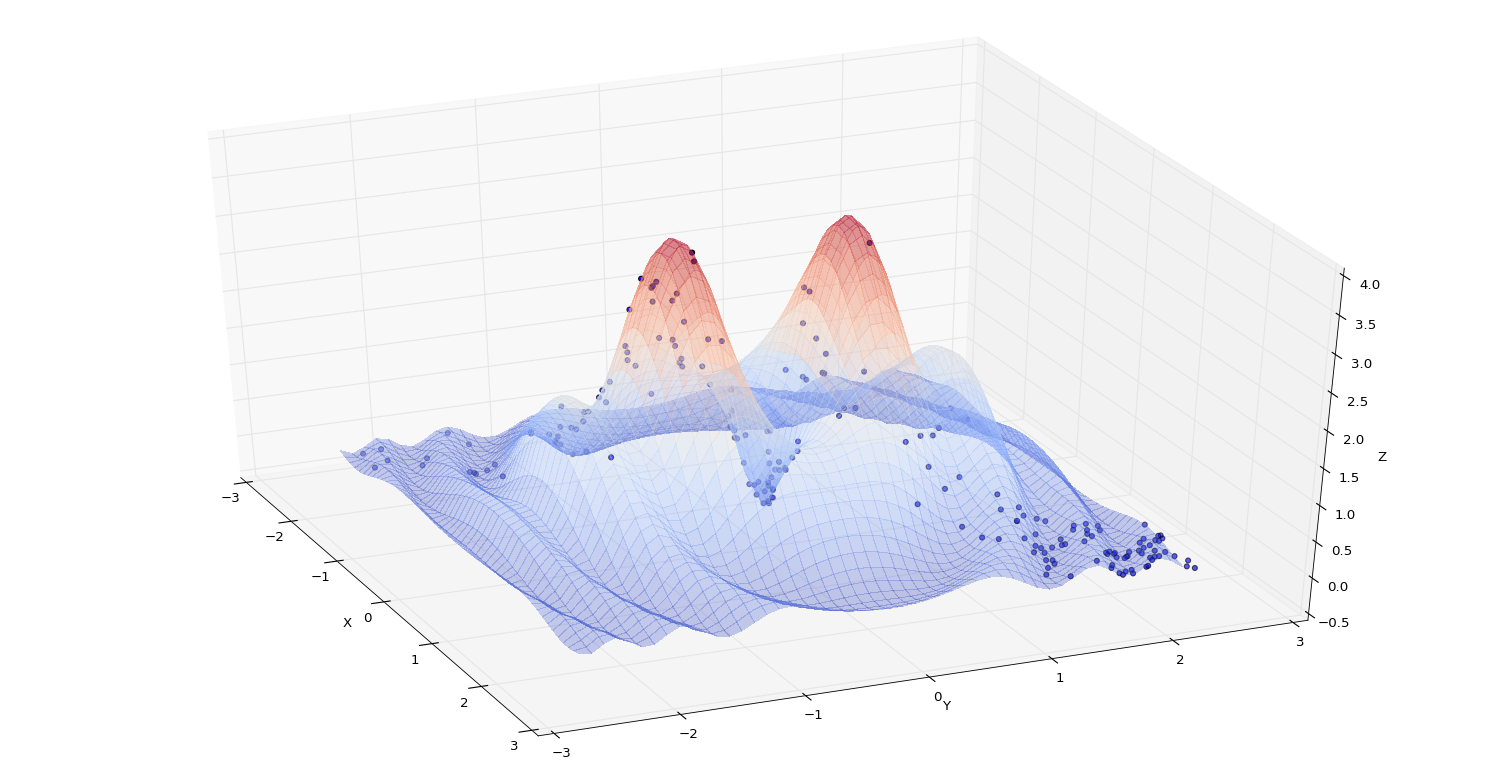
\includegraphics[width=\linewidth]{simulated_annealing.png}
      \caption{Simulated annealing with neighborhood radius of 0.5, starting temperature of 100, and temp *= .975 after each iteration}
      \label{fig:graph1}
   \end{figure}

\end{document}